%%%%%%%%%%%%%%%%%%%%%%%%%%%%%%%%%%%%%%%%%%%%%%%%%%%%%%%%%%%`
%% Supporting Information
%%
%% TODO: Free energy corrections to OER intermediates, OER mechanism
%%%%%%%%%%%%%%%%%%%%%%%%%%%%%%%%%%%%%%%%%%%%%%%%%%%%%%%%%%%


% #########################################################
\section{Active Learning ML Section}  % ###################
% #########################################################
%
% #########################################################
% | - Active Learning ML Section

% %%%%%%%%%%%%%%%%%%%%%%%%%%%%%%%%%%%%%%%%%%%%%%%%%%%%%%%%%
\subsection{Candidate space generation}  % %%%%%%%%%%%%%%%%
% %%%%%%%%%%%%%%%%%%%%%%%%%%%%%%%%%%%%%%%%%%%%%%%%%%%%%%%%%
%
% %%%%%%%%%%%%%%%%%%%%%%%%%%%%%%%%%%%%%%%%%%%%%%%%%%%%%%%%%
% | - Candidate space generation


% %%%%%%%%%%%%%%%%%%%%%%%%%%%%%%%%%%%%%%%%%%%%%%%%%%%%%%%%%
% | - Candidate Generation Intro
% Basic intro into candidate generation
% High-level overview again
%   * Data mining OQMD MP fro AB2/3 entries
%   * Reduce data set by eliminating structurally redundant systems
%     * This is done with Ankit's scheme
% __|
% %%%%%%%%%%%%%%%%%%%%%%%%%%%%%%%%%%%%%%%%%%%%%%%%%%%%%%%%%
% | - PARAGRAPH BODY
%
Here we describe the methodology to construct the set of structural candidates in more detail.
%
The first step of the procedure is to mine materials databases for entries with the desired non-element specific stoichiometry (\latin{i.e.} \ABtwo and \ABthree).
%
Since many of the entries in these databases are structurally redundant,
we used a structure classification scheme to reduce the data set to a structurally unique set.
%
Once this is accomplished, the elements of interest were then substituted into the database structures,
which at this point had their original elemental composition from their database.
%
Finally, the structures are isotropically expanded or contracted to accommodate the difference between the atomic radii of the original elements in the structure and the user defined elements.
%
This procedure of ``pre-optimization'' is an important because it generates reasonable initial geometries which would otherwise produce poor fingerprint representations and lead to a large degree of structural shift during the course of DFT optimization.s
% __|
%%%%%%%%%%%%%%%%%%%%%%%%%%%%%%%%%%%%%%%%%%%%%%%%%%%%%%%%%%%


% %%%%%%%%%%%%%%%%%%%%%%%%%%%%%%%%%%%%%%%%%%%%%%%%%%%%%%%%%
% | - TEMP
% Data-mining OQMD and MP
% __|
% %%%%%%%%%%%%%%%%%%%%%%%%%%%%%%%%%%%%%%%%%%%%%%%%%%%%%%%%%
% | - PARAGRAPH BODY
%Herein, we take advantage of the structural diversity already present in materials databases to construct our candidates.
%
We utilized two materials databases, the Open Quantum Materials (OQMD) and the Materials Project (MP) databases because of their large and diverse datasets of crystalline inorganic materials.
%
% TODO Approx. when did Ankit parse these databases
At the time that we originally mined these databases (2018), there were \num{61471} inorganic compounds in the MP database and \num{435583} entries in the OQMD database.
%
We note that the databases have expanded the number of entries considerably since we originally parsed them,
although the number of unique crystal polymorphs is not expected to have increase significantly.
% __|
%%%%%%%%%%%%%%%%%%%%%%%%%%%%%%%%%%%%%%%%%%%%%%%%%%%%%%%%%%%


% %%%%%%%%%%%%%%%%%%%%%%%%%%%%%%%%%%%%%%%%%%%%%%%%%%%%%%%%%
% | - TEMP
%
% __|
% %%%%%%%%%%%%%%%%%%%%%%%%%%%%%%%%%%%%%%%%%%%%%%%%%%%%%%%%%
% | - PARAGRAPH BODY
%
The structural classification scheme of Jain \latin{et al.} was used assign the crystal prototype, consisting of standardized spacegroup and Wyckoff positions, as well as the element-nonspecific stoichiometry of each structure (\num{497054} in total). This prototype designation can serve as a structural fingerprint and has successfully been applied towards the prediction of formation energies of inorganic compounds \cite{Jain2018}.
%
% COMBAK Revise if Ankit's scheme becomes it's own section
% If it's not ready now, let's not include it.
%See section TEMP for more details on the symmetry based structural classification scheme.
%
Once classified, we selected all entries with the desired stoichiometry of \ABtwo and \ABthree,
for which MP has \num{2424} and \num{2341} \ABtwo and \ABthree entries, respectively,
and OQMD has \num{4736} and \num{28883} \ABtwo and \ABthree entries, respectively.
%
The reason that there are considerably more \ABthree compounds in OQMD is due to the extensive compositional permutation of binary alloys in a cubic \ABthree structure.
%
Within each stoichiometry, the structural classification was used to eliminate structurally redundant systems,
\latin{i.e.} systems that share their stoichiometry, space-group, and Wyckoff positions.
%
This process reduces the data set to \num{620} and \num{219} unique structures of \ABtwo and \ABthree for MP and \num{397} and \num{194} structurally unique \ABtwo and \ABthree OQMD entries.
%
Combining the MP and OQMD data sets ultimately results in a dataset of \num{688} \ABtwo and \num{254} \ABthree structurally unique candidates.
% __|
%%%%%%%%%%%%%%%%%%%%%%%%%%%%%%%%%%%%%%%%%%%%%%%%%%%%%%%%%%%


% =========================================================
% TABLE ===================================================
% =========================================================
% | - Table | OQMD MP Structures
\begin{table}[!htb]

  \caption{\label{table:database_structures}
    %
    (a) Number of entries in the OQMD and MP materials databases for the \ABtwo and \ABthree stoichiometries.
    %
    (b) Final number of unique structural candidates for \ABtwo and \ABthree.
    }
  %
  % | - Subtable a
  \begin{subtable}{.5\linewidth}
  \centering
  \caption{}
  %
   %
    %
    \begin{tabular}{cccc}
    \textbf{}         & \textbf{}        & \multicolumn{2}{c}{\textbf{Entries}} \\
    \textbf{Database} & \textbf{Stoich.} & \textbf{Total}   & \textbf{Unique}   \\
    OQMD              &                  & 435,583          &                   \\
                      & \ABtwo           & 4,736            & 397               \\
                      & \ABthree         & 28,883           & 194               \\
    \hline
    MP                &                  & 61,471           &                   \\
                      & \ABtwo           & 2,424            & 620               \\
                      & \ABthree         & 2,341            & 219
    \end{tabular}
    %
   %
  %
  \end{subtable}
  % __|
  %
  %
  \newline
  \vspace*{0.8 cm}
  \newline
  %
  %
  % | - Subtable b
  \begin{subtable}{.5\linewidth}
  \centering
  \caption{}
  %
   %
    %
    \begin{tabular}{cc}
    \multicolumn{2}{c}{\textbf{Final Candidate Set}} \\
    \textbf{Stoich.}   & \textbf{Unique Structures}  \\
    \ABtwo             & 697                         \\
    \ABthree           & 259
    \end{tabular}
    %
   %
  %
  \end{subtable}
  % __|
  %
\end{table}
% __| =====================================================
% =========================================================

% __|


% %%%%%%%%%%%%%%%%%%%%%%%%%%%%%%%%%%%%%%%%%%%%%%%%%%%%%%%%%
\subsection{Structure featurization and data processing}  %
% %%%%%%%%%%%%%%%%%%%%%%%%%%%%%%%%%%%%%%%%%%%%%%%%%%%%%%%%%
%
% %%%%%%%%%%%%%%%%%%%%%%%%%%%%%%%%%%%%%%%%%%%%%%%%%%%%%%%%%
% | - Structure featurization and data processing


% %%%%%%%%%%%%%%%%%%%%%%%%%%%%%%%%%%%%%%%%%%%%%%%%%%%%%%%%%
% | - TEMP
%
% __|
% %%%%%%%%%%%%%%%%%%%%%%%%%%%%%%%%%%%%%%%%%%%%%%%%%%%%%%%%%
% | - PARAGRAPH BODY
%
Structures are featurized using the Voronoi tessellation method developed by Ward et al. \cite{Ward2017}.
Zero-variance features that don't encode for any information within a set of structures with constant composition and stoichiometry are removed before model training, reducing the number of feature columns from \num{271} to \num{101}.
%
The number of features are further reduced to \num{10} by performing a principal component analysis (PCA). The optimal number of principle components was found by computing the cross-validation MAE on the post-relaxation fingerprints as a function of PCA components (Figure \ref{fig:cv_anal}),
where it was found that 10 PCA components is sufficient to minimize the error.
% TODO Add all of the feature engineering steps here
% __|
%%%%%%%%%%%%%%%%%%%%%%%%%%%%%%%%%%%%%%%%%%%%%%%%%%%%%%%%%%%


% __|


% =========================================================
% FIGURE ==================================================
% | - Figure | Cross-validation analysis ******************
\begin{figure*}[!htb]
\centering
\makebox[\textwidth][c]{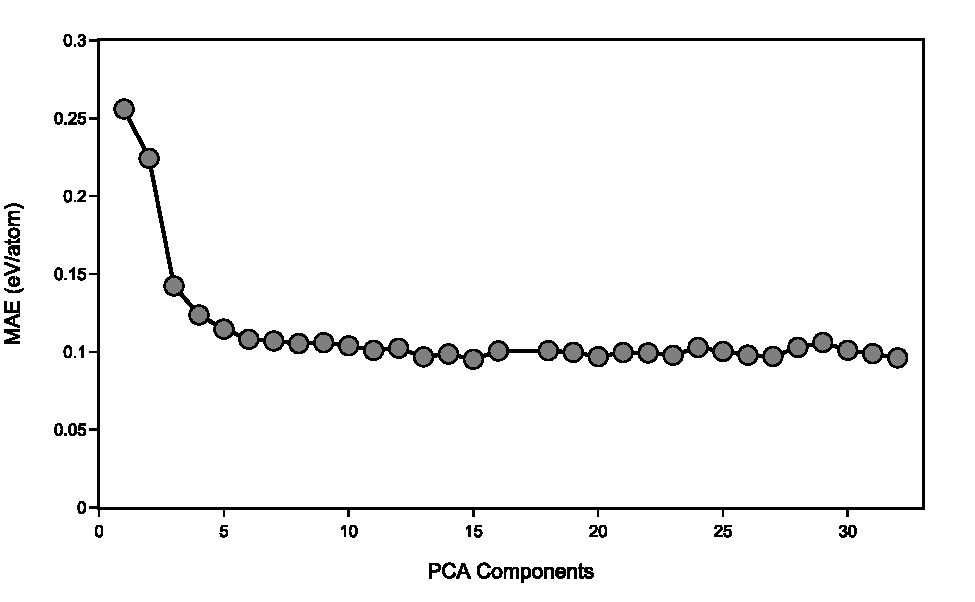
\includegraphics
{02_figures/SI_figures/00_mae_pca_plot__v0.pdf}}
\caption{\label{fig:cv_anal}
20-fold cross validation mean absolute error (MAE) as a function of the number of PCA components used for the GP-regression for \IrOthree. Only post-relaxation fingerprints were used for both training and testing to avoid issues with structural drift. All structural duplicates in the post-relaxation dataset were removed.
}
\end{figure*}
% __|
% =========================================================


% %%%%%%%%%%%%%%%%%%%%%%%%%%%%%%%%%%%%%%%%%%%%%%%%%%%%%%%%%
\subsection{Gaussian process regression model}  % %%%%%%%%%
% %%%%%%%%%%%%%%%%%%%%%%%%%%%%%%%%%%%%%%%%%%%%%%%%%%%%%%%%%
% Relevant details about the ML Gaussian process here
%
% %%%%%%%%%%%%%%%%%%%%%%%%%%%%%%%%%%%%%%%%%%%%%%%%%%%%%%%%%
% | - Gaussian process regression model


% %%%%%%%%%%%%%%%%%%%%%%%%%%%%%%%%%%%%%%%%%%%%%%%%%%%%%%%%%
% | - TEMP
%
% __|
% %%%%%%%%%%%%%%%%%%%%%%%%%%%%%%%%%%%%%%%%%%%%%%%%%%%%%%%%%
% | - PARAGRAPH BODY
%
Gaussian process machine learning regression models were picked due to their highly flexible fits and high performance in situations with small data sets. We utilized the Gaussian Process regression module as implemented in CatLearn.\cite{hansen2019atomistic,CatLearn_Repo} The Gaussian Process recipe we developed utilized two isotropic Gaussian kernels which differ only in the value of the initial length scale parameter, $l$: \textbf{Raul:isn't the scaling optimized for each of them, so that $s$ is also different? Also please add noise kernel in equation below.}

\begin{equation}
    k(x,x') = s_1 exp \Bigl ( \frac{-|x-x'|^2}{2l_1^2}\Bigr) + s_2 exp\Bigl(\frac{-|x-x'|^2}{2l_2^2}\Bigr) + NOISE-kernel?
\end{equation}


Here, isotropic refers to keeping the dimensionality of the kernel equal to one instead of an anisotropic kernel which was found to be difficult to optimize.
%
The first GP kernel was constructed with a length scale parameter of 1 while for the second kernel the length scale was reduced by a factor of ten (0.1). This was done with the aim of producing a model that is responsive to both long- and short-range features in the input space. Additionally, the noise parameter, $TEMP$, was set to a value of \num{0.025}, the scaling parameters, $s_1$, $s_2$ and $\alpha$ was set to 5.2.
%
% TODO Double check that I said it correctly, might be minimizing the LML
These initial value for the hyper-parameters of the GP kernel are then optimized during every training round,
which occurs once per active learning loop,
and is done by maximizing the log marginal likelihood of the model and training data.
% __|
%%%%%%%%%%%%%%%%%%%%%%%%%%%%%%%%%%%%%%%%%%%%%%%%%%%%%%%%%%%





% __|


% %%%%%%%%%%%%%%%%%%%%%%%%%%%%%%%%%%%%%%%%%%%%%%%%%%%%%%%%%
\subsection{Bulk polymorph DFT optimization}  % %%%%%%%%%%%
% %%%%%%%%%%%%%%%%%%%%%%%%%%%%%%%%%%%%%%%%%%%%%%%%%%%%%%%%%
% VASP
% PBE exchange correlation functional
% spin-polarized calculations
% plane-wave cutoff of 600 eV
% %%%%%%%%%%%%%%%%%%%%%%%%%%%%%%%%%%%%%%%%%%%%%%%%%%%%%%%%%
% | - Bulk polymorph DFT optimization


% %%%%%%%%%%%%%%%%%%%%%%%%%%%%%%%%%%%%%%%%%%%%%%%%%%%%%%%%%
% | - TEMP
%
% __|
% %%%%%%%%%%%%%%%%%%%%%%%%%%%%%%%%%%%%%%%%%%%%%%%%%%%%%%%%%
% | - PARAGRAPH BODY
%
All DFT calculations were performed using density functional theory (DFT) implemented via the Vienna \latin{ab-initio} simulation package (VASP) \cite{Kresse1995,Kresse1996_0,Kresse1996_1} and utilizing the PBE exchange-correlation functional\cite{Perdew1996}. A cutoff plane-wave cutoff of 600 eV was used, and calculations were spin-polarized. A variable k-point mesh was used such that a k-point density of at least \num{20} k-points per reciprocal space dimension.
%
All bulk systems were run through the following computational recipe to converge the equilibrium structure, with \num{3} distinct phases. structures are only advanced to the next phase when the previous phase completes without error.
\\
1. An ISIF \num{7} calculation to optimize only the volume (initial volume of cell may be really off).
\\
2. Three consecutive ISIF \num{3} relaxations to fully converge the lattice and atomic positions.
\\
3. A final ISIF \num{2} calculation to relax the atomic coordinates only to avoid errors associated with changing the cell volume with a fixed plane-wave cutoff basis.
\\
The final ISIF \num{2} step is run with an electronic energy SCF convergence criteria of \SI{1e-6} eV and the ionic relaxation has a tight force convergence criteria of \SI{1e-3}{\electronvolt\per\angstrom}.
% __|
%%%%%%%%%%%%%%%%%%%%%%%%%%%%%%%%%%%%%%%%%%%%%%%%%%%%%%%%%%%


% __|


% %%%%%%%%%%%%%%%%%%%%%%%%%%%%%%%%%%%%%%%%%%%%%%%%%%%%%%%%%
\subsection{\IrOtwo Active Learning Results} %
% %%%%%%%%%%%%%%%%%%%%%%%%%%%%%%%%%%%%%%%%%%%%%%%%%%%%%%%%%
% Here are the analogous IrO2 results that were presented for IrO3 in the main text
% %%%%%%%%%%%%%%%%%%%%%%%%%%%%%%%%%%%%%%%%%%%%%%%%%%%%%%%%%
% | - IrO2 Active Learning Results


% %%%%%%%%%%%%%%%%%%%%%%%%%%%%%%%%%%%%%%%%%%%%%%%%%%%%%%%%%
% | - TEMP
%
% __|
% %%%%%%%%%%%%%%%%%%%%%%%%%%%%%%%%%%%%%%%%%%%%%%%%%%%%%%%%%
% | - PARAGRAPH BODY
%
TEMP section about IrO2 active learning results.
% __|
%%%%%%%%%%%%%%%%%%%%%%%%%%%%%%%%%%%%%%%%%%%%%%%%%%%%%%%%%%%


% __|


% =========================================================
% FIGURE ==================================================
% =========================================================
% | - Figure | IrO2 Active Learning Results
\begin{figure*}[!htb]
\centering
\makebox[\textwidth][c]{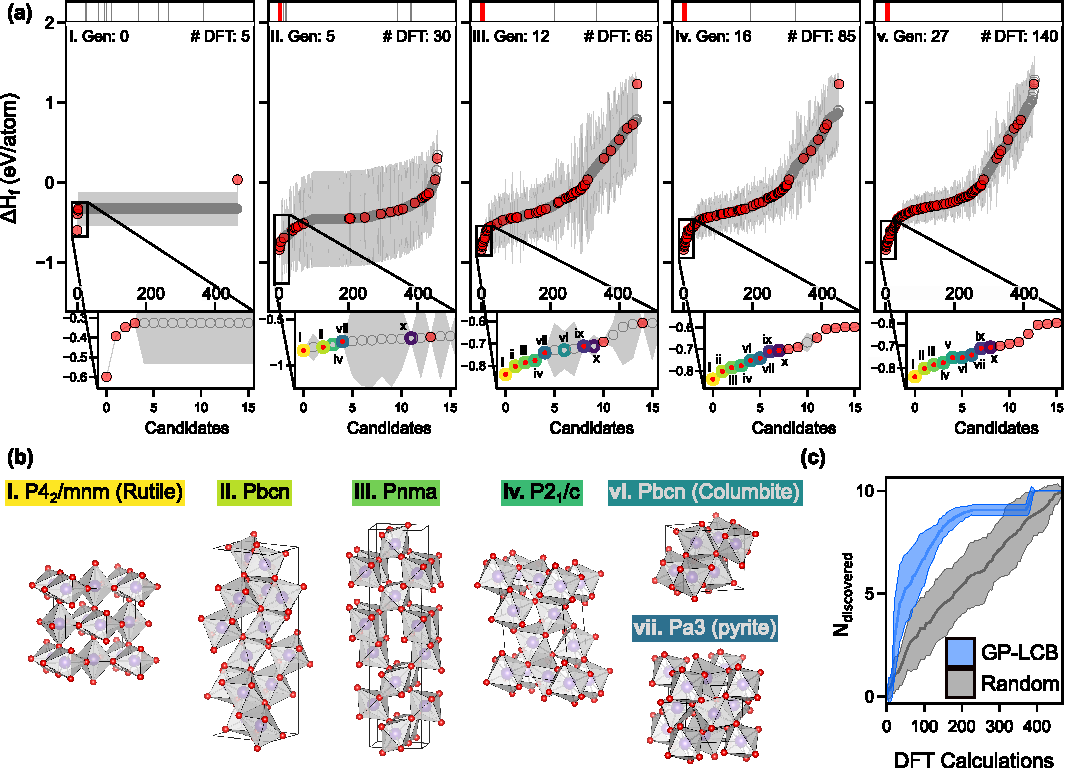
\includegraphics
{02_figures/SI_figures/00_ml_plot_iro2_al__v7__downsampled_1000x1000.pdf}}
\caption{\label{fig:iro2_al}
%
Results for the active learning algorithm applied to the \IrOtwo space.
%
Analogous to Figure \ref{fig:iro3_al}, see Figure \ref{fig:iro3_al} for description of all subplots.
}
\end{figure*}
% __| =====================================================
% =========================================================


% %%%%%%%%%%%%%%%%%%%%%%%%%%%%%%%%%%%%%%%%%%%%%%%%%%%%%%%%%
\subsection{Discovery rate of all runs of AL algorithms} %%
% %%%%%%%%%%%%%%%%%%%%%%%%%%%%%%%%%%%%%%%%%%%%%%%%%%%%%%%%%
% TEMP
% %%%%%%%%%%%%%%%%%%%%%%%%%%%%%%%%%%%%%%%%%%%%%%%%%%%%%%%%%
% | - Discovery rate of all runs of AL algorithms


% %%%%%%%%%%%%%%%%%%%%%%%%%%%%%%%%%%%%%%%%%%%%%%%%%%%%%%%%%
% | - TEMP
%
% __|
% %%%%%%%%%%%%%%%%%%%%%%%%%%%%%%%%%%%%%%%%%%%%%%%%%%%%%%%%%
% | - PARAGRAPH BODY
%
TEMP section
% __|
%%%%%%%%%%%%%%%%%%%%%%%%%%%%%%%%%%%%%%%%%%%%%%%%%%%%%%%%%%%


% __|


% =========================================================
% FIGURE ==================================================
% =========================================================
% | - Figure | Discovery rate of all runs of AL algorithms
\begin{figure*}[!htb]
\centering
\makebox[\textwidth][c]{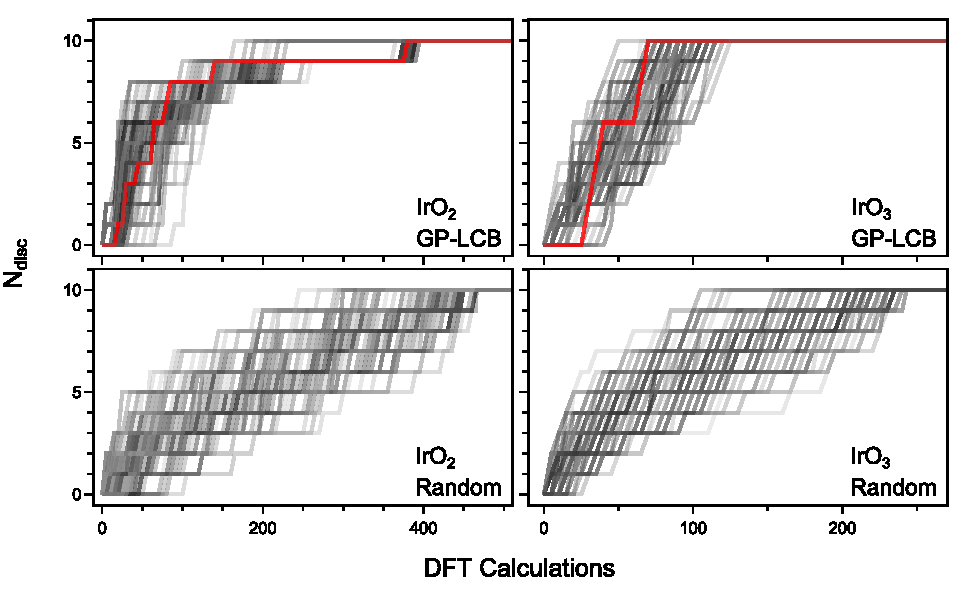
\includegraphics
{02_figures/SI_figures/00_disc_vs_dft__v1.pdf}}
\caption{\label{fig:disc_rate}
%
Quantity of top ten most stable \IrOtwo and \IrOthree polymorphs discovered ($N_{disc}$) as a function of the number of DFT bulk optimizations performed for the GP-LCB acquisition and the baseline random acquisition methods.
%
Red lines indicate the specific runs used for Figures \ref{fig:iro3_al} and Figure \ref{fig:iro2_al}.
}
\end{figure*}
% __| =====================================================
% =========================================================


% %%%%%%%%%%%%%%%%%%%%%%%%%%%%%%%%%%%%%%%%%%%%%%%%%%%%%%%%%
\subsection{Structural coordination motif identification} %
% %%%%%%%%%%%%%%%%%%%%%%%%%%%%%%%%%%%%%%%%%%%%%%%%%%%%%%%%%
%
% %%%%%%%%%%%%%%%%%%%%%%%%%%%%%%%%%%%%%%%%%%%%%%%%%%%%%%%%%
% | - Structural coordination motif identification


% %%%%%%%%%%%%%%%%%%%%%%%%%%%%%%%%%%%%%%%%%%%%%%%%%%%%%%%%%
% | - TEMP
%
% __|
% %%%%%%%%%%%%%%%%%%%%%%%%%%%%%%%%%%%%%%%%%%%%%%%%%%%%%%%%%
% | - PARAGRAPH BODY
TEMP section about doing the structural motiff analysis. Maybe not needed.
% __|
%%%%%%%%%%%%%%%%%%%%%%%%%%%%%%%%%%%%%%%%%%%%%%%%%%%%%%%%%%%


% __|


% %%%%%%%%%%%%%%%%%%%%%%%%%%%%%%%%%%%%%%%%%%%%%%%%%%%%%%%%%
\subsection{Amorphous phase meta-stability analysis} %%%%%%
% %%%%%%%%%%%%%%%%%%%%%%%%%%%%%%%%%%%%%%%%%%%%%%%%%%%%%%%%%
%
% %%%%%%%%%%%%%%%%%%%%%%%%%%%%%%%%%%%%%%%%%%%%%%%%%%%%%%%%%
% | - Amorphous phase meta-stability analysis

% %%%%%%%%%%%%%%%%%%%%%%%%%%%%%%%%%%%%%%%%%%%%%%%%%%%%%%%%%
% | - TEMP
%
% __|
% %%%%%%%%%%%%%%%%%%%%%%%%%%%%%%%%%%%%%%%%%%%%%%%%%%%%%%%%%
% | - PARAGRAPH BODY
The meta-stability analysis based on an ensemble of meta-stable phases developed by TEMP was utlized to set a physically motivated energy cut-off relative to the hull to evaluate the synthesizability of our hypothetical polymorphs.
% __|
%%%%%%%%%%%%%%%%%%%%%%%%%%%%%%%%%%%%%%%%%%%%%%%%%%%%%%%%%%%

% __|

% __|


% #########################################################
\section{Electrochemical OER Computational Methods}  % ####
% #########################################################
%
% #########################################################
% | - Electrochemical OER Computational Methods

% %%%%%%%%%%%%%%%%%%%%%%%%%%%%%%%%%%%%%%%%%%%%%%%%%%%%%%%%%
\subsection{Density Functional Theory Methods}  % %%%%%%%%%
% %%%%%%%%%%%%%%%%%%%%%%%%%%%%%%%%%%%%%%%%%%%%%%%%%%%%%%%%%
%
% %%%%%%%%%%%%%%%%%%%%%%%%%%%%%%%%%%%%%%%%%%%%%%%%%%%%%%%%%
% | - Density Functional Theory Methods
%
All OER calculations were performed using density functional theory (DFT) implemented via the Vienna \latin{ab-initio} simulation package (VASP)
\cite{Kresse1995,Kresse1996_0,Kresse1996_1}
and utilizing the PBE exchange-correlation functional\cite{Perdew1996}.
%
Dipole corrections were imposed on all non-symmetric slabs to counteract spurious dipole interactions between the periodic cells.\cite{Neugebauer1992}
%
% TODO COMBAK, make this section more general, k-points were treated differently
% for different calculations
A 4x4x3 k-point mesh with gamma-point centered Monkshort-packing\cite{Monkhorst1976} was used for all slabs.
%
The plane-wave energy cutoff was \SI{500}{\electronvolt}.
%
% COMBAK Figure out how much spacing was used for all slabs
All slab calculations maintained a vacuum spacing in between TEMP and \SI{15}{\angstrom}
%
All structures were relaxed with utilizing the conjugate gradient algorithm as implemented in VASP (IBRION\num{=2}).
%
The simulation stop criteria used was that all atoms must satisfy a maximum force threshold of \SI{0.02}{\electronvolt\per\angstrom}.
% __|


% %%%%%%%%%%%%%%%%%%%%%%%%%%%%%%%%%%%%%%%%%%%%%%%%%%%%%%%%%
\subsection{Bulk Pourbaix Diagram}  % %%%%%%%%%%%%%%%%%%%%%
% %%%%%%%%%%%%%%%%%%%%%%%%%%%%%%%%%%%%%%%%%%%%%%%%%%%%%%%%%
%
% %%%%%%%%%%%%%%%%%%%%%%%%%%%%%%%%%%%%%%%%%%%%%%%%%%%%%%%%%
% | - Bulk Pourbaix Diagram
%
The electrochemical bulk Pourbaix diagrams were constructed using the TEMP module from pymatgen.
% __|


% =========================================================
% FIGURE ==================================================
% =========================================================
% | - Figure | Bulk Pourbaix Diagram
\begin{figure*}[!htb]
\centering
\makebox[\textwidth][c]{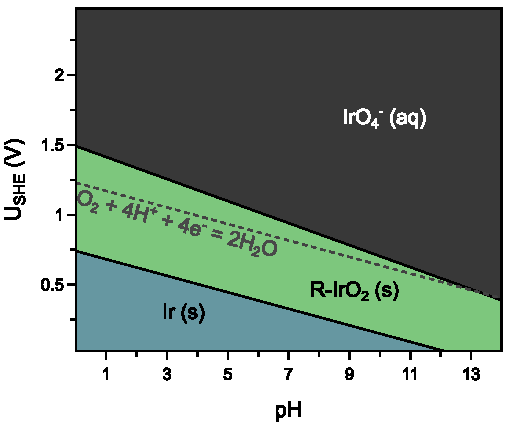
\includegraphics
{02_figures/SI_figures/00_master__bulk-pourbaix__v5.pdf}}
\caption{\label{fig:bulk_pourbaix_wo_alpha}
%
Bulk Pourbaix diagram of the \ce{Ir}-\ce{H2O} system as a function of the applied potential and pH.
%
The diagram was constructed using all of the same species as Figure \ref{fig:bulk_pourbaix} with the exception of the globally stable \IrOthree (\aIrOthree) polymorph.
%
%
% Revised bulk Pourbaix diagram of the \ce{Ir}-\ce{H2O} system as a function of applied potential and pH.
% %
% The diagram was constructed with Ir(s) (blue), \rIrOtwo (green), various \IrOthree polymorphs and a dissolved \ce{IrO^{4-}} ion species (dark grey).
% %
% The stability regions corresponding to the metastable \rIrOthree and \bIrOthree polymorphs, in the absence of any competing \IrOthree phase, are displayed as yellow and pink lines, respectively.
% %
% The thermodynamic onset of OER (water equilibrium at 1.23 \VRHE) is also shown.
}
\end{figure*}
% __| =====================================================
% =========================================================


% %%%%%%%%%%%%%%%%%%%%%%%%%%%%%%%%%%%%%%%%%%%%%%%%%%%%%%%%%
\subsection{OER Thermodynamic Methodology}  % %%%%%%%%%%%%%
% %%%%%%%%%%%%%%%%%%%%%%%%%%%%%%%%%%%%%%%%%%%%%%%%%%%%%%%%%
%
% %%%%%%%%%%%%%%%%%%%%%%%%%%%%%%%%%%%%%%%%%%%%%%%%%%%%%%%%%
% | - OER Thermodynamic Methodology
%
Here we will outline the procedure used to carry out OER simulations on the various slabs of \IrOtwo and \IrOthree.
%
The procedure was as follows:
%
Stable stoichiometric terminations were cut from the bulk.
%
% COMBAK
% TODO Add Vesta reference
Stable termination planes were guesstimated via intuition, and the x-ray diffraction pattern tool from Vesta.
%
Next, electrochemical surface coverage was elucidated via a surface Pourbaix analysis.
%
This elucidates the coverage under operating conditions ($>$\num{1.23} \VRHE) for each slab.
%
% COMBAK
Finally we conducted a thermodynamic/limiting potential analysis of the OER mechanistic pathway (Volcano plot, limiting potentials, etc.).
% __|


% %%%%%%%%%%%%%%%%%%%%%%%%%%%%%%%%%%%%%%%%%%%%%%%%%%%%%%%%%
\subsection{Surface Energy Pourbaix Methodology}  % %%%%%%%
% %%%%%%%%%%%%%%%%%%%%%%%%%%%%%%%%%%%%%%%%%%%%%%%%%%%%%%%%%
%
% %%%%%%%%%%%%%%%%%%%%%%%%%%%%%%%%%%%%%%%%%%%%%%%%%%%%%%%%%
% | - Surface Energy Pourbaix Methodology
%
Surface energy Pourbaix plots were constructed by calculating the surface energy of each slab by under standard conditions (\si{\volt}\num{=0} and pH\num{=0}) and then utilizing the computational hydrogen electrode (CHE) to compute the potential dependence of the surfaces.
%
Surface energy calculations were performed for various facets for slabs of increasing thickness.
%
% TODO Insert reference for surface E calcs
The bulk energy was then extracted by fitting the total energy of the slabs against the number of layers as explained in TEMP.
%
This was  done to avoid common issues of surface energy divergence associated with using a separate bulk energy calculation.
%
The sensitivity of a given slab to an applied bias is dependent on the composition of the surface,
in particular, the effect of coverage of electrolyte species which can deposit oxygen, hydrogen, and hydroxide species on the surface layers.
%
These additional \ce{O} and \ce{H} atoms are not referenced to the atoms in the slab, but are instead referenced to the computational hydrogen electrode and water-splitting reaction.
%
% TODO Type out equations for surface energy calculation
The equation for is as follows:
% __|


% %%%%%%%%%%%%%%%%%%%%%%%%%%%%%%%%%%%%%%%%%%%%%%%%%%%%%%%%%
\subsection{OER Scaling Relations}  % %%%%%%%%%%%%%%%%%%%%%
% %%%%%%%%%%%%%%%%%%%%%%%%%%%%%%%%%%%%%%%%%%%%%%%%%%%%%%%%%
%
% %%%%%%%%%%%%%%%%%%%%%%%%%%%%%%%%%%%%%%%%%%%%%%%%%%%%%%%%%
% %%%%%%%%%%%%%%%%%%%%%%%%%%%%%%%%%%%%%%%%%%%%%%%%%%%%%%%%%
% | - OER Scaling Relations


% %%%%%%%%%%%%%%%%%%%%%%%%%%%%%%%%%%%%%%%%%%%%%%%%%%%%%%%%%
% | - TEMP
%
% __|
% %%%%%%%%%%%%%%%%%%%%%%%%%%%%%%%%%%%%%%%%%%%%%%%%%%%%%%%%%
% | - PARAGRAPH BODY
%
Figure~\ref{fig:scaling_relations} shows the scaling relations between the adsorption free energies of the OER intermediate species for the studied \IrOx slabs.
%
It can be seen clearly that the data points corresponding to the three \IrOthree polymorphs are roughly \SI{1}{\electronvolt} weaker binding than the \rIrOtwo points.
%
This generally weaker binding of the \IrOthree stoichiometry is responsible for the observed improvement in theoretical activity.
%
The \DGOOH vs.\DGOH relationship is very close to the traditional ``universal scaling relations'', demonstrating that our materials do not break the infamous \DGOOH vs. \DGOH scaling.

% __|
%%%%%%%%%%%%%%%%%%%%%%%%%%%%%%%%%%%%%%%%%%%%%%%%%%%%%%%%%%%


% __|


% =========================================================
% FIGURE ==================================================
% =========================================================
% | - Figure | OER Scaling Relations
\begin{figure*}[!htb]
\centering
\makebox[\textwidth][c]{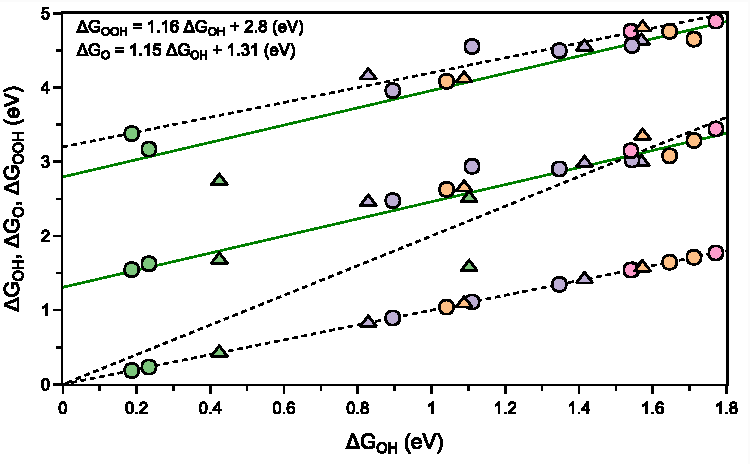
\includegraphics
{02_figures/SI_figures/00_master__oer_scaling__main_v3.pdf}}
\caption{\label{fig:scaling_relations}
%
Relationship between the adsorption free energies of the three key OER intermediates (*OH, *O, *OOH), with \DGOH chosen as the dependent variable.
%
Best fit lines are provided for \DGOOH vs. \DGOH and \DGO vs. \DGOH.
%
Additionally, ``universal scaling relations'' for \DGOOH vs. \DGOH and \DGO vs. \DGOH are shown (black dotted lines) to emphasize our deviation from the traditionally reported scaling fits.
%
The \DGOH line is  shown as guide to eye.
% TODO Do I have to redefine the color convention every caption?
}
\end{figure*}
% __| =====================================================
% =========================================================


% %%%%%%%%%%%%%%%%%%%%%%%%%%%%%%%%%%%%%%%%%%%%%%%%%%%%%%%%%
\subsection{Bulk Systems}  % %%%%%%%%%%%%%%%%%%%%%%%%%%%%%%
% %%%%%%%%%%%%%%%%%%%%%%%%%%%%%%%%%%%%%%%%%%%%%%%%%%%%%%%%%
%
% %%%%%%%%%%%%%%%%%%%%%%%%%%%%%%%%%%%%%%%%%%%%%%%%%%%%%%%%%
% %%%%%%%%%%%%%%%%%%%%%%%%%%%%%%%%%%%%%%%%%%%%%%%%%%%%%%%%%
% | - Bulk Systems


% %%%%%%%%%%%%%%%%%%%%%%%%%%%%%%%%%%%%%%%%%%%%%%%%%%%%%%%%%
% | - TEMP
%
% __|
% %%%%%%%%%%%%%%%%%%%%%%%%%%%%%%%%%%%%%%%%%%%%%%%%%%%%%%%%%
% | - PARAGRAPH BODY
% Formation energies of 4 polymorphs
% __|
%%%%%%%%%%%%%%%%%%%%%%%%%%%%%%%%%%%%%%%%%%%%%%%%%%%%%%%%%%%


% __|


% %%%%%%%%%%%%%%%%%%%%%%%%%%%%%%%%%%%%%%%%%%%%%%%%%%%%%%%%%
\subsection{Table of OER energetics}  % %%%%%%%%%%%%%%%%%%%
% %%%%%%%%%%%%%%%%%%%%%%%%%%%%%%%%%%%%%%%%%%%%%%%%%%%%%%%%%
%
% %%%%%%%%%%%%%%%%%%%%%%%%%%%%%%%%%%%%%%%%%%%%%%%%%%%%%%%%%
% %%%%%%%%%%%%%%%%%%%%%%%%%%%%%%%%%%%%%%%%%%%%%%%%%%%%%%%%%
% | - Table of OER energetics


% %%%%%%%%%%%%%%%%%%%%%%%%%%%%%%%%%%%%%%%%%%%%%%%%%%%%%%%%%
% | - TEMP
%
% __|
% %%%%%%%%%%%%%%%%%%%%%%%%%%%%%%%%%%%%%%%%%%%%%%%%%%%%%%%%%
% | - PARAGRAPH BODY
%
Table \ref{table:oer_data} contains the adsorbate binding energetics for the intermediates of the OER
oxygen evolution reaction (*O, *OOH, *OH).
% __|
%%%%%%%%%%%%%%%%%%%%%%%%%%%%%%%%%%%%%%%%%%%%%%%%%%%%%%%%%%%


% __|


% =========================================================
% TABLE ===================================================
% =========================================================
% | - Table | OER energetics
\newpage  % request a new page.
\begin{landscape}
\renewcommand{\arraystretch}{1.5} % <--------------
\begin{table}
\resizebox{\linewidth}{!}{%
\centering
\caption{\label{table:oer_data}
%
OER adsorbation energies for slabs of \IrOtwo and \IrOthree polymorphs studied here.
%
Included quantities are electronic adsorption energies
($\Delta E_{*O_{x}H_{y}}$),
adsorption free energies
($\Delta G_{*O_{x}H_{y}}$),
as well as the \DGOmOH OER descriptor.
%
Coverage indicates the electrochemical coverage of either *O or *OH species.
%
The limiting potential and corresponding overpotential ($\eta$) as well as the rate determining step (RDS) for the OER mechanism are shown.
}
\begin{tabular}{lllcccccccccc}
\toprule
                Bulk Sys. &    Facet &    Coverage & $\Delta E_{*OH}$ & $\Delta E_{*O}$ & $\Delta E_{*OOH}$ & $\Delta G_{*OH}$ & $\Delta G_{*O}$ & $\Delta G_{*OOH}$ & $\Delta G_{*O}-\Delta G_{*OH}$ & Lim. Pot. & $\eta$ &                                                                    RDS \\
                        - &        - &           - &             (eV) &            (eV) &              (eV) &             (eV) &            (eV) &              (eV) &                           (eV) &       (V) &    (V) &                                                                      - \\
\midrule
      $R{\text -}IrO_{2}$ &    (100) &         *OH &            0.130 &           1.634 &             2.362 &            0.424 &           1.678 &             2.738 &                          1.254 &     2.182 &  0.952 &              $*OOH \rightarrow * \phantom{T} \phantom{T} \phantom{T} $ \\
      $R{\text -}IrO_{2}$ &    (100) &          *O &           -0.061 &           1.582 &             2.793 &            0.234 &           1.626 &             3.170 &                          1.392 &     1.750 &  0.520 &              $*OOH \rightarrow * \phantom{T} \phantom{T} \phantom{T} $ \\
      $R{\text -}IrO_{2}$ &    (110) &         *OH &            0.807 &           1.535 &             2.133 &            1.102 &           1.579 &             2.509 &                          0.477 &     2.411 &  1.181 &              $*OOH \rightarrow * \phantom{T} \phantom{T} \phantom{T} $ \\
      $R{\text -}IrO_{2}$ &    (110) &          *O &           -0.108 &           1.503 &             3.004 &            0.187 &           1.547 &             3.380 &                          1.360 &     1.833 &  0.603 &                         $*O \phantom{T} \phantom{T}  \rightarrow *OOH$ \\
 $\alpha{\text -}IrO_{3}$ &    (100) &         *OH &            1.275 &           2.950 &             4.254 &            1.569 &           2.994 &             4.630 &                          1.424 &     1.636 &  0.406 &                         $*O \phantom{T} \phantom{T}  \rightarrow *OOH$ \\
 $\alpha{\text -}IrO_{3}$ &    (100) &          *O &            1.249 &           2.980 &             4.191 &            1.544 &           3.024 &             4.567 &                          1.480 &     1.544 &  0.314 &  $* \phantom{T} \phantom{T} \phantom{T}  \rightarrow *OH \phantom{T} $ \\
 $\alpha{\text -}IrO_{3}$ &    (110) &         *OH &            0.534 &           2.414 &             3.786 &            0.828 &           2.458 &             4.163 &                          1.629 &     1.705 &  0.475 &                         $*O \phantom{T} \phantom{T}  \rightarrow *OOH$ \\
 $\alpha{\text -}IrO_{3}$ &    (110) &          *O &            0.600 &           2.432 &             3.582 &            0.895 &           2.476 &             3.959 &                          1.581 &     1.581 &  0.351 &              $*OH \phantom{T} \rightarrow *O \phantom{T} \phantom{T} $ \\
 $\alpha{\text -}IrO_{3}$ &    (111) &          *O &            0.815 &           2.894 &             4.177 &            1.110 &           2.938 &             4.554 &                          1.828 &     1.828 &  0.598 &              $*OH \phantom{T} \rightarrow *O \phantom{T} \phantom{T} $ \\
 $\alpha{\text -}IrO_{3}$ &    (211) &         *OH &            1.120 &           2.937 &             4.173 &            1.415 &           2.981 &             4.549 &                          1.566 &     1.568 &  0.338 &                         $*O \phantom{T} \phantom{T}  \rightarrow *OOH$ \\
 $\alpha{\text -}IrO_{3}$ &    (211) &          *O &            1.052 &           2.860 &             4.122 &            1.347 &           2.904 &             4.499 &                          1.558 &     1.594 &  0.364 &                         $*O \phantom{T} \phantom{T}  \rightarrow *OOH$ \\
  $\beta{\text -}IrO_{3}$ &  (010)-A &          *O &            1.246 &           3.105 &             4.383 &            1.541 &           3.149 &             4.759 &                          1.609 &     1.610 &  0.380 &                         $*O \phantom{T} \phantom{T}  \rightarrow *OOH$ \\
  $\beta{\text -}IrO_{3}$ &  (010)-B &          *O &            1.477 &           3.399 &             4.519 &            1.771 &           3.443 &             4.896 &                          1.672 &     1.771 &  0.541 &  $* \phantom{T} \phantom{T} \phantom{T}  \rightarrow *OH \phantom{T} $ \\
      $R{\text -}IrO_{3}$ &    (100) &         *OH &            1.278 &           3.304 &             4.431 &            1.572 &           3.348 &             4.807 &                          1.776 &     1.776 &  0.546 &              $*OH \phantom{T} \rightarrow *O \phantom{T} \phantom{T} $ \\
      $R{\text -}IrO_{3}$ &    (100) &          *O &            1.351 &           3.036 &             4.381 &            1.646 &           3.080 &             4.758 &                          1.435 &     1.677 &  0.447 &                         $*O \phantom{T} \phantom{T}  \rightarrow *OOH$ \\
      $R{\text -}IrO_{3}$ &    (100) &  *O-partial &            1.417 &           3.243 &             4.275 &            1.712 &           3.287 &             4.652 &                          1.575 &     1.712 &  0.482 &  $* \phantom{T} \phantom{T} \phantom{T}  \rightarrow *OH \phantom{T} $ \\
      $R{\text -}IrO_{3}$ &    (110) &         *OH &            0.794 &           2.607 &             3.744 &            1.088 &           2.651 &             4.121 &                          1.563 &     1.563 &  0.333 &              $*OH \phantom{T} \rightarrow *O \phantom{T} \phantom{T} $ \\
      $R{\text -}IrO_{3}$ &    (110) &          *O &            0.746 &           2.583 &             3.708 &            1.041 &           2.627 &             4.084 &                          1.586 &     1.586 &  0.356 &              $*OH \phantom{T} \rightarrow *O \phantom{T} \phantom{T} $ \\
\bottomrule
\end{tabular}

}
\end{table}

\end{landscape}
% __| =====================================================
% =========================================================

% __|
